\section{Backend}

The following section describes how the Erlang NetInf streaming functionality was evaluated and tested. 

\subsection{Video streaming protocol evaluation}
One of the problems discussed was reducing congestion when broadcasting content. 
This was solved by implementing an alternative way of sending chunked data as seen in 
Section \ref{sec:Chunkeddata} according to the video streaming draft in 
Appendix C \ref{VideoDraft}. In the following section this implementation is referred to
as the \textit{modified streaming}. 
The following tests were conducted:

\begin{itemize}
\item Testing the modified version of NetInf video streaming. 
\item Testing the pure version of NetInf video streaming.
\item Comparison between both implementations of the NetInf Video streaming
\end{itemize}

The testing was done by transferring 500 chunks of bogus data between a number of different NetInf nodes running the NRS. 
All the receiving nodes started the transfer at the same time.
To be able to publish $N$ number of chunks in an easy and fast manner, the \textit{nn\_evaluation} module was implemented.

\subsection{Pure video streaming evaluation setup}
The nodes that were included in the pure version of the streaming were the following:
Central NRS node, one streaming source node that published all 500 NDOs to itself with 
\textit{fullput} set to True, then also published the NDO to the central NRS with 
\textit{fullput} set to False. The central NRS can not have the octets 
because otherwise it would provide all clients with the octets directly, 
hence prevent the network load to be more balanced.

Five client nodes then retrieved each chunk by:
\begin{enumerate}
\item searching NRS for the chunk with chunk number and stream name.
\item getting the NDO metadata and locators from the NRS.
\item fetching NDO with octects from one of the locators.
\item publishing the NDO to itself 
\item adding itself as a locator and publish to the NRS.
\item repeating the procedure for the next chunk.
\end{enumerate}

\subsection{Modified video streaming evaluation setup}
In this setup one node served both as the source and central NRS while there 
were five other client nodes. The source first published the stream NDO to itself, 
then used the content dispatcher to put all the chunks into the storage.
The clients then get the streamed NDO, added themselves as 
locator and published it to the NRS. To retrieve the chunks each client need to:

\begin{enumerate}
\item append the current chunk number to the NDO name.
\item send the request to one of the locators.
\item if status of the response is 404, repeat step 2.
\item store the octects in its storage.
\item increase the chunk number
\end{enumerate}

\subsection{Results} 
The Figure~\ref{fig:eval-stream-modvspure} shows 
that the pure NetInf streaming is faster when it comes to 
transferring all the chunks. 

The CPU load of the central NRS was recorded with the built in system monitor, 
the result of the pure version is in Figure~\ref{fig:eval-stream-pure-cpu} and the modified in Figure~\ref{fig:eval-stream-mod-cpu}. 


\begin{figure}[h!]
	\centering
		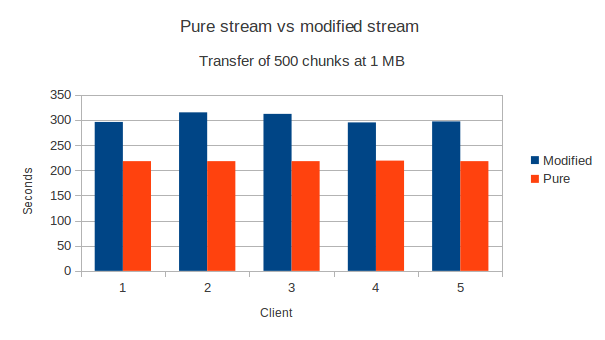
\includegraphics[width=0.75\textwidth]{./img/eval-stream-plot-modvspure.png}
    	\caption{Pure streaming vs modified streaming}
	\label{fig:eval-stream-modvspure}
\end{figure}

\begin{figure}[h!]
	\centering
		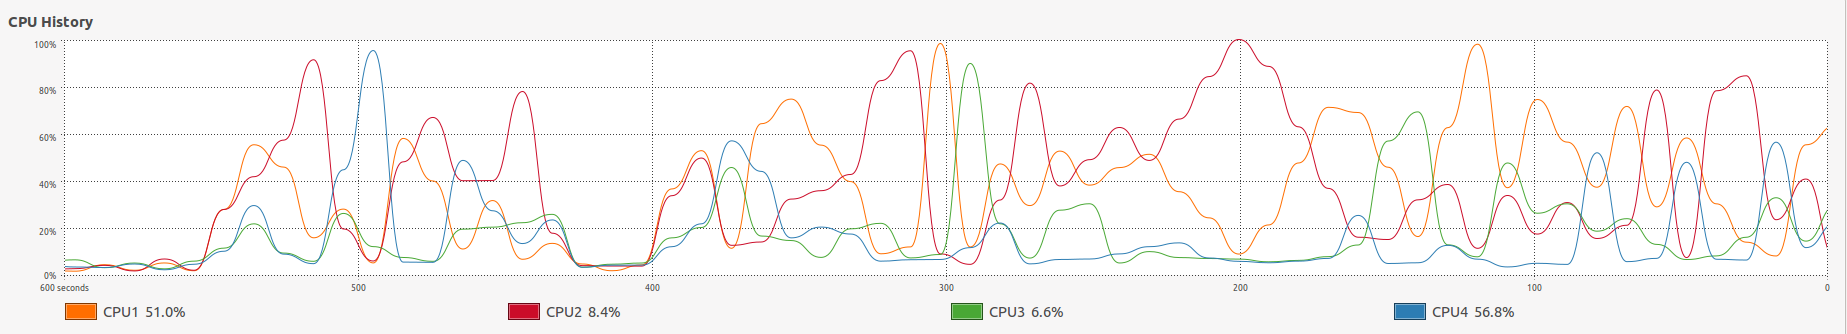
\includegraphics[width=0.75\textwidth]{./img/eval-stream-pure-cpu.png}
    	\caption{Central NRS CPU usage during pure streaming}
	\label{fig:eval-stream-pure-cpu}
\end{figure}

\begin{figure}[h!]
	\centering
		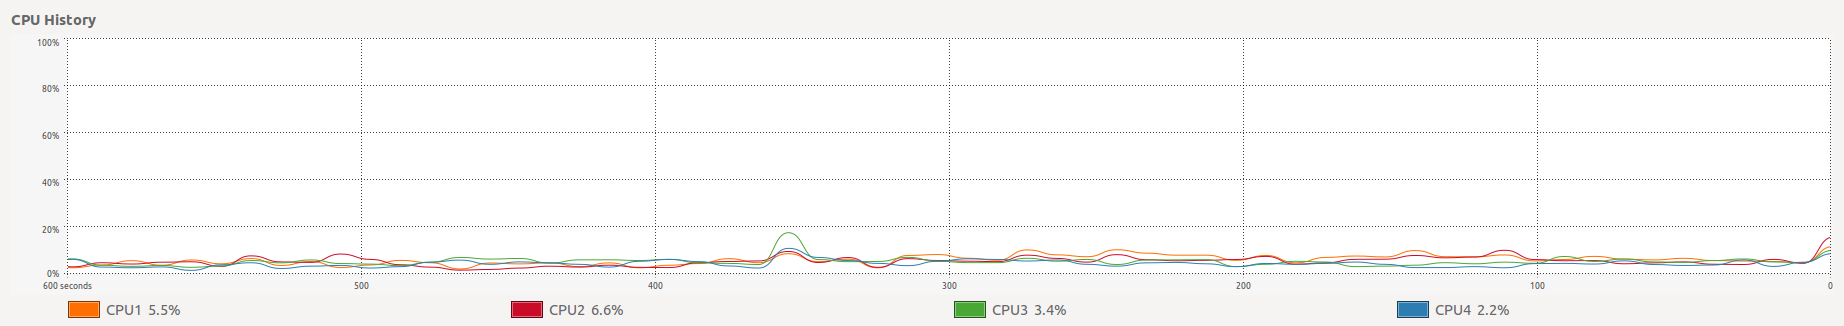
\includegraphics[width=0.75\textwidth]{./img/eval-stream-mod-cpu.png}
    	\caption{Central NRS CPU usage during modified streaming}
	\label{fig:eval-stream-mod-cpu}
\end{figure}

\subsection{Discussion}
As can be seen in Figure~\ref{fig:eval-stream-modvspure} the transfer of the chunks 
took less time using the pure streaming, this was not unexpected since the modified version has a lot of overhead in this case, 
if it tries to get chunks from another client which does not have them yet, 
this will yield an 404 response and the client will need to try another source. 
The pure NetInf however will get a hit every time. 

Comparing CPU load in Figure~\ref{fig:eval-stream-pure-cpu} and Figure~\ref{fig:eval-stream-mod-cpu}, 
shows that even with only five receiving nodes the pure central NRS was under considerably high load.
While in the modified versions load was almost not noticeable. The CPU load on the pure NRS is caused by  
the number of database lookups. 

\subsection{Notes on Interoperability}

There are already existing implementations created by SAIL and Ericsson Research 
for the NetInf protocol\citation{netinfproto}. In the beginning of the product 
life-cycle the customer requested the development team to evaluate the interoperability 
of this product with other systems. However as the product evolved the customer requested 
that the interoperability be left to them to evaluate and that this development team 
continue with evaluating the video streaming instead.

Therefore the development team did not evaluate interoperability, but there is confidence
that with minor tweaking of the code (due to differences in the various draft versions of
the NetInf protocol specification) this product and others will become interoperable.

The following list describes the evaluation performed for testing the NetInf NRS application.

\begin{itemize}
\item Evaluation of the search time and get time for the supported databases
\item Measuring the number of requests per frontend phone client
\end{itemize}
